\documentclass[12pt, a4paper]{article}
\usepackage{graphicx} % Required for inserting images
\usepackage[paper=a4paper,top=1in,bottom=1in,right=1in,left=1in]{geometry}% http://ctan.org/pkg/geometry
\usepackage{amsmath, xparse}
\setcounter{MaxMatrixCols}{20}
\usepackage{caption}
\usepackage[framed, numbered]{matlab-prettifier}
\usepackage{longtable}
\usepackage{float}
\usepackage{amsmath}
\usepackage{comment}
\usepackage{mismath}
\newcommand{\eqnum}{\refstepcounter{equation}\tag{\theequation}}


\setlength\parindent{0pt}
\numberwithin{equation}{section}



\begin{document}

\begin{titlepage}
   \begin{center}
       
\includegraphics[width=0.25\textwidth]{img/metu.png}\\
       \vspace*{1cm}
       \Large
       \textbf{MIDDLE EAST TECHNICAL UNIVERSITY}\\
       \vspace{0.05cm}
       \textbf{DEPARTMENT OF MECHANICAL ENGINEERING}\\
       \vspace{1.2cm}
       \textbf{ME 310 – NUMERICAL METHODS}\\
       \textbf{SPRING 2022}\\
       \vspace{3cm}
       \text{HOMEWORK 2}\\
       \vspace{2cm}
       \text{Muhammed Rüstem ŞEVİK - 2446888}

       \vfill
       
       \small
       I understand that this is an individual assignment. I affirm that I have not given or received
any unauthorized help on this assignment, and that this work is my own.
            
       \vspace{0cm}

            
   \end{center}
\end{titlepage}

\newpage
    \renewcommand{\contentsname}{Table of Contents}
    \tableofcontents
    \listoffigures
    \listoftables
\newpage

\section{Introduction}
In this report, we will methodically address a series of numerical problems through the application of specialized computational techniques. Initially, we shall employ Gauss quadrature integration to evaluate a specific integral and contrast its accuracy with alternative methodologies, namely the multiple segment trapezoidal rule, and Simpson’s 1/3 and 3/8 rules. Additionally, an investigation into MATLAB's quad function will shed light on its operational mechanics. Following this, the report will embark on an exploration of rocket dynamics, utilizing Romberg integration to ascertain the maximum altitude attained by a rocket based on its propulsive characteristics. Furthermore, the analysis will extend to the study of heat flux in a fin with given temperature distribution data, employing numerical differentiation to determine the rate of change of temperature, and subsequently, the heat flux. Lastly, the focus will shift to the evaluation of an aircraft's motion based on recorded data. By employing finite difference methods to approximate the derivatives, the report will facilitate the calculation and graphical representation of the aircraft’s velocity and acceleration profiles. MATLAB will serve as the primary tool for implementing the calculations and graphical representations throughout the report.

\section{Body}
\subsection{Question 2}


\subsubsection{Part A}

Evaluate the following integral using Gauss quadrature integration with 4 points and weights.


\begin{equation}
\int_{0}^{2\pi} x \sin(x) dx
\end{equation}

The formula for Gauss quadrature integration is given by:

\begin{equation}
    \int_{a}^{b} f(x) dx \approx \frac{b-a}{2} \sum_{i=1}^{n} w_i f\left(\frac{b-a}{2} x_i + \frac{a+b}{2}\right)
\end{equation}



where \(a\) and \(b\) are the limits of integration, \(n\) is the number of points, \(w_i\) are the weights, and \(x_i\) are the coordinates.\\

In this case, we have \(a = 0\), \(b = 2\pi\), \(n = 4\)

Using the provided coordinates and weights, we have:

\begin{align*}
\text{Point 1:} \quad & x_1 = -0.8611363115940526, \quad w_1 = 0.3478548451374539 \\
\text{Point 2:} \quad & x_2 = -0.3399810435848563, \quad w_2 = 0.6521451548625461 \\
\text{Point 3:} \quad & x_3 = +0.3399810435848563, \quad w_3 = 0.6521451548625461 \\
\text{Point 4:} \quad & x_4 = +0.8611363115940526, \quad w_4 = 0.3478548451374539 \\
\end{align*}

Using these values, we can evaluate the integral:

\begin{align}
\int_{0}^{2\pi} x \sin(x) dx \approx \frac{2\pi-0}{2} [w_1 f\left(\frac{2\pi-0}{2} x_1 + \frac{0+2\pi}{2}\right) \notag \\
\quad + w_2 f\left(\frac{2\pi-0}{2} x_2 + \frac{0+2\pi}{2}\right) \notag \\
\quad + w_3 f\left(\frac{2\pi-0}{2} x_3 + \frac{0+2\pi}{2}\right)  \\
\quad + w_4 f\left(\frac{2\pi-0}{2} x_4 + \frac{0+2\pi}{2}\right)] \notag
\end{align}

Substituting the given values into the formula, we get:

\begin{align}
\approx \frac{2\pi - 0}{2} [0.3478548451374539 \cdot f\left(\frac{2\pi - 0}{2}(-0.8611363115940526) + \frac{2\pi + 0}{2}\right) \notag \\
\quad + 0.6521451548625461 \cdot f\left(\frac{2\pi - 0}{2}(-0.3399810435848563) + \frac{2\pi + 0}{2}\right) \\
\quad + 0.6521451548625461 \cdot f\left(\frac{2\pi - 0}{2}(0.3399810435848563) + \frac{2\pi + 0}{2}\right) \notag \\
\quad + 0.3478548451374539 \cdot f\left(\frac{2\pi - 0}{2}(0.8611363115940526) + \frac{2\pi + 0}{2}\right)] \notag
\end{align}

Evaluating this gives the Gauss quadrature approximation as approximately 

\begin{equation}
\int_{0}^{2\pi} x \sin(x) dx \approx -6.333516813159698
\end{equation}

To find the true error, we need to calculate the exact value of the integral. Let's integrate \(x \sin(x)\) with respect to \(x\). We can use MATLAB.


\begin{equation}
\int_{0}^{2\pi} x \sin(x) dx = -6.283185228932334
\end{equation}

Comparing this with the approximated value from Gauss quadrature integration, we can find the true error:

\[
\text{True error} = \text{Exact value} - \text{Approximated value}
\]

The true error becomes

\[
\text{True error} = 0.050331584227364
\]



\subsubsection{Part B}
The formula is:
\begin{equation}
    \int_a^b f(x) \, dx \approx \frac{h}{2} \left[ f(a) + 2 \sum_{i=1}^{n-1} f(x_i) + f(b) \right]
\end{equation}
For the true error to fall under the same true error, the number of iterations required for using the multiple segment trapezoidal rule

\[
\text{Number of iterations} = 21
\]

\subsubsection{Part C}
The formula is:
\begin{equation}
\int_a^b f(x) \, dx \approx \frac{h}{3} \left[ f(x_0) + 4 \sum_{i=1}^{n/2} f(x_{2i-1}) + 2 \sum_{i=1}^{n/2-1} f(x_{2i}) + f(x_n) \right]
\end{equation}

For the true error to fall under the same true error, the number of iterations required for using the multiple segment Simpson’s 1/3 rule

\[
\text{Number of iterations} = 6
\]
\subsubsection{Part D}
\begin{equation}
    \int_a^b f(x) \, dx \approx \frac{3h}{8} \left[ f(x_0) + 3 \sum_{i=1}^{n/3} f(x_{3i-2}) + 3 \sum_{i=1}^{n/3} f(x_{3i-1}) + 2 \sum_{i=1}^{n/3-1} f(x_{3i}) + f(x_n) \right]
\end{equation}
\\
For the true error to fall under the same true error, the number of iterations required for using the multiple segment Simpson’s 3/8 rule

\[
\text{Number of iterations} = 9
\]
\subsubsection{Part E}

MATLAB's `quad` function is a powerful tool for numerical integration, which calculates the definite integral of a function between two specified limits. The function employs an adaptive quadrature method that is based on Simpson's rule. This method begins by approximating the integral using a low-order formula and then refines this approximation in an iterative manner until the error estimate falls below a certain specified tolerance or the maximum number of iterations is reached. The `quad` function requires three primary inputs: the function to be integrated, and the lower and upper limits of integration. The function to be integrated can be defined in two ways: either inline using the '@(x)' syntax, or as a separate function file. The lower and upper limits of integration are simply the two points between which the definite integral of the function is to be calculated. In addition to these primary inputs, the `quad` function also accepts optional parameters that can be used to control aspects of the computation. For example, the 'AbsTol' and 'RelTol' parameters can be used to specify the absolute and relative error tolerances for the computation. The 'MaxIntervalCount' parameter can be used to limit the maximum number of intervals that the function will use in the computation. These optional parameters provide a high level of control over the computation, making the `quad` function a versatile and powerful tool for numerical integration. It is particularly useful for integrating functions that can be evaluated at an arbitrary number of points, and it is efficient for functions that are smooth over the interval of integration.

\newpage
\subsubsection{Code}
\lstinputlisting[style=Matlab-editor, basicstyle=\mlttfamily\scriptsize]{Q2.m}

\newpage
\subsection{Question 4}

\subsubsection{Methodology}
To solve this problem, we need to integrate the velocity function over the time interval from 0 to 30 seconds. This will give us the total distance traveled by the rocket, which is the height it will reach. The Romberg integration method is a numerical integration technique that can be used to approximate the definite integral of a function.

The velocity function given in the problem is:

\begin{equation}
v(t) = v_f \ln\left(\frac{m_0}{m_0 - qt}\right) - gt
\end{equation}

where:
\(v_f = 1500 \, \text{m/s}\) is the velocity at which fuel is expelled relative to the rocket,
\(m_0 = 1.5 \times 10^5 \, \text{kg}\) is the initial mass of the rocket,
\(q = 2300 \, \text{kg/s}\) is the fuel consumption rate,
\(g = 9.81 \, \text{m/s}^2\) is the acceleration due to gravity, and
\(t\) is the time.\\

To find the height \(h\) the rocket will reach in 30 seconds, we need to integrate the velocity function from 0 to 30:

\begin{equation}
h = \int_{0}^{30} v(t) \, dt
\end{equation}

We can use the Romberg integration method to approximate this integral. Romberg integration is a method that uses the trapezoidal rule at step-sizes related by a power of two and then performs Richardson extrapolation on these results to approximate the integral with a higher degree of accuracy. The trapezoidal rule is a method for approximating the definite integral of a function. It works by approximating the region under the graph of the function as a trapezoid and calculating its area. The formula for the trapezoidal rule is:

\begin{equation}
T(h) = \frac{h}{2} \left[f(a) + 2\sum_{i=1}^{n-1} f(a+ih) + f(b)\right]    
\end{equation}


where \(h = (b-a)/n\) is the width of each subinterval, \(a\) and \(b\) are the limits of integration, and \(n\) is the number of subintervals.\\

In our case, \(a = 0\), \(b = 30\), and we'll start with \(n = 1\). We'll compute \(T(h)\) for \(h = 30, 15, 7.5, 3.75\).\\

The Romberg approximations \(R(i, j)\) are computed using the following formula:

\begin{equation}
R(i, j) = R(i, j-1) + \frac{1}{4^{j-1}-1} \left[R(i, j-1) - R(i-1, j-1)\right]    
\end{equation}


where \(R(i, j-1)\) and \(R(i-1, j-1)\) are the previously computed Romberg approximations.\\

We repeat the process until the difference between successive approximations is less than a specified tolerance, or until we have computed a specified number of approximations.\\
\begin{table}[H]
    \centering
    \caption{Romberg integration table}
    \begin{tabular}{c|c|ccc} \hline
        $h$ & $O(h^2)$ & $O(h^4)$ & $O(h^6)$ & $O(h^8)$ \\ \hline
        30 & $T(30)$ & & &  \\
        15 & $T(15)$ & $R(1, 1)$ & &  \\
        7.5 & $T(7.5)$ & $R(2, 1)$ & $R(2, 2)$ &  \\
        3.75 & $T(3.75)$ & $R(3, 1)$ & $R(3, 2)$ & $R(3, 3)$ \\ \hline
    \end{tabular}
    \label{tab:my_label}
\end{table}

\\

For \(h = 30\):

\begin{equation}
T(30) = \frac{30}{2} \left[v(0) + v(30)\right]
\end{equation}

For \(h = 15\):

\begin{equation}
T(15) = \frac{15}{2} \left[v(0) + 2v(15) + v(30)\right]
\end{equation}

For \(h = 7.5\):

\begin{equation}
T(7.5) = \frac{7.5}{2} \left[v(0) + 2v(7.5) + 2v(15) + 2v(22.5) + v(30)\right]
\end{equation}

For \(h = 3.75\):

\begin{align}
T(3.75) = \frac{3.75}{2} [v(0) + 2v(3.75) + 2v(7.5) + 2v(11.25) + 2v(15) + 2v(18.75) \\ \notag
\quad + 2v(22.5) + 2v(26.25) + v(30)]
\end{align}

Compute the Romberg approximations:

For \(i = 1, j = 1\):

\begin{equation}
R(1, 1) = T(15) + \frac{1}{4^{1}-1} \left[T(15) - T(30)\right]
\end{equation}

For \(i = 2, j = 1\):

\begin{equation}
R(2, 1) = T(7.5) + \frac{1}{4^{1}-1} \left[T(7.5) - T(15)\right]
\end{equation}

For \(i = 3, j = 1\):

\begin{equation}
R(3, 1) = T(3.75) + \frac{1}{4^{1}-1} \left[T(3.75) - T(7.5)\right]
\end{equation}

For \(i = 2, j = 2\):

\begin{equation}
R(2, 2) = R(2, 1) + \frac{1}{4^{2}-1} \left[R(2, 1) - R(1, 1)\right]
\end{equation}

For \(i = 3, j = 2\):

\begin{equation}
R(3, 2) = R(3, 1) + \frac{1}{4^{2}-1} \left[R(3, 1) - R(2, 1)\right]
\end{equation}

For \(i = 3, j = 3\):

\begin{equation}
R(3, 3) = R(3, 2) + \frac{1}{4^{3}-1} \left[R(3, 2) - R(2, 2)\right]
\end{equation}

The numerical solutions for the trapezoidal approximations \(T(h)\) and the Romberg approximations \(R(i, j)\) are:

For \(h = 30\):

  $$T(30) \approx 9449.69 \, \text{m}$$

For \(h = 15\):

  $$T(15) \approx 8398.30 \, \text{m}$$

For \(h = 7.5\):

  $$T(7.5) \approx 8126.39 \, \text{m}$$

For \(h = 3.75\):

  $$T(3.75) \approx 8057.74 \, \text{m}$$

Compute the Romberg approximations:

For \(i = 1, j = 1\):

  $$R(1, 1) \approx 8398.30 \, \text{m}$$

For \(i = 2, j = 1\):

  $$R(2, 1) \approx 8126.39 \, \text{m}$$

For \(i = 3, j = 1\):

  $$R(3, 1) \approx 8057.74 \, \text{m}$$

For \(i = 2, j = 2\):

  $$R(2, 2) \approx 8035.75 \, \text{m}$$

For \(i = 3, j = 2\):

  $$R(3, 2) \approx 8034.86 \, \text{m}$$

For \(i = 3, j = 3\):

  $$R(3, 3) \approx 8034.80 \, \text{m}$$

So, the completed table is:

\begin{table}[H]
    \centering
    \caption{Numerical values for Romberg integration table}
    \begin{tabular}{ccccc} \hline
        $h$ & $O(h^2)$ & $O(h^4)$ & $O(h^6)$ & $O(h^8)$ \\ \hline
        30 & 9449.69 & & &  \\
        15 & 8398.30 & 8398.30 & &  \\
        7.5 & 8126.39 & 8126.39 & 8035.75 &  \\
        3.75 & 8057.74 & 8057.74 & 8034.86 & 8034.80 \\ \hline
    \end{tabular}
\end{table}

The rocket will reach a height of approximately 8034.80 meters in 30 seconds according to the Romberg integration method.

\newpage
\newpage
\subsection{Question 8}

The 2-point forward difference derivative approximation formula:

\begin{equation}
f'(x_0) \approx \frac{{f(x_1) - f(x_0)}}{{\Delta x}}
\end{equation}

The 3-point forward difference derivative approximation formula:

\begin{equation}
f'(x_0) \approx \frac{{-3f(x_0) + 4f(x_1) - f(x_2)}}{{2\Delta x}}    
\end{equation}

In this formula, $f'(x_0)$ represents the approximation of the derivative of the function at $x_0$. The function values at the points $x_0$, $x_1$, $x_2$, and $x_3$ are denoted as $f(x_0)$, $f(x_1)$, $f(x_2)$, and $f(x_3)$ respectively. $\Delta x$ represents the spacing between these points.\\

The 2-point backward difference derivative approximation formula:

\begin{equation}
f'(x_n) \approx \frac{{f(x_n) - f(x_{n-1})}}{{\Delta x}}
\end{equation}

The 3-point backward difference derivative approximation formula:

\begin{equation}
f'(x_n) \approx \frac{{3f(x_n) - 4f(x_{n-1}) + f(x_{n-2})}}{{2\Delta x}}
\end{equation}

In these formulas, \(f'(x_n)\) represents the approximation of the derivative of the function at \(x_n\). The function values at the points \(x_n\), \(x_{n-1}\), \(x_{n-2}\), and \(x_{n-3}\) are denoted as \(f(x_n)\), \(f(x_{n-1})\), \(f(x_{n-2})\), and \(f(x_{n-3})\) respectively. \(\Delta x\) represents the spacing between these points.Note that the subscripts \(n-1\), \(n-2\), and \(n-3\) indicate points preceding \(x_n\), as these formulas are for backward difference approximation.\\

Derivation of the 4 point differentiation formulas

\begin{align}
& f(x+\Delta x)=f(x)+f^{\prime}(x) \cdot \Delta x+f^{\prime \prime}(x) \cdot \frac{(\Delta x)^{2}}{2}+f^{\prime \prime \prime}(x) \cdot \frac{(\Delta x)^{3}}{6}+\bigO(\Delta x)^{4} \\
& f(x+2 \Delta x)=f(x)+f^{\prime}(x) \cdot 2 \Delta x+f^{\prime \prime}(x) \cdot 4\frac{ (\Delta x)^{2}}{2}+f^{\prime \prime \prime}(x) \cdot 8 \frac{(\Delta x)^{3}}{6}+\bigO(\Delta x)^{4} \\
& f(x+3 \Delta x)=f(x)+f^{\prime}(x) \cdot 3 \Delta x+f^{\prime \prime}(x) \cdot 9\frac{(\Delta x)^{2}}{2}+f^{\prime \prime \prime}(x) \cdot 27 \frac{(\Delta x)^{3}}{6}+\bigO(\Delta x)^{4} 
\end{align}

Multiply the equations with approptiate factors
\begin{align}
18[f\left(x_{1}\right) =& f(x)+f^{\prime}(x) \cdot \Delta x+f^{\prime \prime}\left(x_{0}\right) \cdot \frac{(\Delta x)^{2}}{2}+f^{\prime \prime \prime}(x_0) \cdot \frac{(\Delta x)^{3}}{6}+\bigO(\Delta x)^{4}] \\
-9[f\left(x_{2}\right) =& f(x)+f^{\prime}(x) \cdot 2 \Delta x+f^{\prime \prime}\left(x_{0}\right) \cdot4 \frac{ \Delta x)^{2}}{2}+f^{\prime \prime \prime}(x_0) \cdot8 \frac{ (\Delta x)^{3}}{6}+\bigO(\Delta x)^{4}] \\
2[f\left(x_{3}\right) =& f(x)+f^{\prime}(x) \cdot 3 \Delta x+f^{\prime \prime}\left(x_{0}\right) \cdot 9\frac{(\Delta x)^{2}}{2}+f^{\prime \prime \prime}(x_0) \cdot 27 \frac{(\Delta x)^{3}}{6}+\bigO(\Delta x)^{4}]
\end{align}
Sum the equations
\begin{equation}
18 f\left(x_{1}\right)-g f\left(x_{2}\right)+2 f\left(x_{0}\right)=11 f\left(x_{0}\right)+6 f^{\prime}\left(x_{0}\right) \Delta x+0+0+\bigO(\Delta x)^{4} 
\end{equation}
Simplify the expression
\begin{equation}
    f^{\prime}\left(x_{0}\right) \approx \frac{18 f\left(x_{1}\right)-g f\left(x_{2}\right)+2 f\left(x_{3}\right)-11 f\left(x_{0}\right)}{6 \Delta x}
\end{equation}
Backward differentiation formula yields

\begin{equation}
    f^{\prime}\left(x_{n}\right) \approx \frac{-18 f\left(x_{n-1}\right)+g f\left(x_{n-2}\right)-2 f\left(x_{n-3}\right)+11 f\left(x_{n}\right)}{6 \Delta x}
\end{equation}

\subsubsection{Part A}

To determine the heat flux at $x = 0$  using 2, 3, and 4 points, we'll use the 2-point forward difference, 3-point forward difference, and 4-point forward difference formulas.\\

\\
\begin{table}[H]
    \centering
    \caption{Given data for temperature differentiation calculations}
    \begin{tabular}{ccccccccccccc} \hline
        $x$[cm] & 0 & 1 & 2 & 3 & 4 & 5 & 6 & 7 & 8 & 9 & 10 \\
        $T$ [K] & 473 & 446.3 & 422.6 & 401.2 & 382 & 364.3 & 348 & 332.7 & 318.1 & 304 & 290.1 \\ \hline
    \end{tabular}
\end{table}

\\
\\

Heat flux at \(x = 0\) using the 2-point forward difference formula:

\begin{equation}
q_0 = -k \cdot \frac{d T}{d x}\Bigg|_{x=0}
\end{equation}

Using the 2-point forward difference formula:

\begin{equation}
\frac{d T}{d x} \approx \frac{T_1 - T_0}{\Delta x}
\end{equation}

where \(\Delta x\) is the spacing between the points. In this case, \(\Delta x = 1\, \text{cm}\) or \(0.01\, \text{m}\). Let's substitute the values:

\begin{equation}
\frac{dT}{dx} \approx \frac{T_1 - T_0}{\Delta x} = \frac{446.3 - 473}{0.01} = -2669.9999\, \text{K/m}
\end{equation}

Now, we can calculate the heat flux:

\begin{equation}
q_0 = -k \cdot \frac{dT}{dx}\Bigg|_{x=0} = -240 \times (-2669.9999) = 640799.9999\, \text{W/m}^2 = 640.8\, \text{kW/m}^2
\end{equation}

Heat flux at \(x = 0\) using the 3-point forward difference formula:

\begin{equation}
q_0 = -k \cdot \frac{d T}{d x}\Bigg|_{x=0}
\end{equation}

Using the 3-point forward difference formula:

\begin{equation}
\frac{d T}{d x} \approx \frac{-3T_0 + 4T_1 - T_2}{2\Delta x}
\end{equation}

Substituting the values:

\begin{equation}
\frac{dT}{dx} \approx \frac{-3T_0 + 4T_1 - T_2}{2\Delta x} = \frac{-3*473 + 4*446.3 - 422.6}{2*0.01} = -2819.9999\, \text{K/m}
\end{equation}

Calculating the heat flux:

\begin{equation}
q_0 = -k \cdot \frac{dT}{dx}\Bigg|_{x=0} = -240 \times (-2819.9999) = 676799.9999\, \text{W/m}^2 = 676.8\, \text{kW/m}^2
\end{equation}

Heat flux at \(x = 0\) using the 4-point forward difference formula:

\begin{equation}
q_0 = -k \cdot \frac{d T}{d x}\Bigg|_{x=0}
\end{equation}

Using the 4-point forward difference formula:

\begin{equation}
\frac{d T}{d x} \approx \frac{18T_1 - 9T_2 + 2T_3 - 11T_0}{6\Delta x}
\end{equation}

Substituting the values:

\begin{equation}
\frac{dT}{dx} \approx \frac{18T_1 - 9T_2 + 2T_3 - 11T_0}{6\Delta x} = \frac{18*446.3 - 9*422.6 + 2*401.2 - 11*473}{6*0.01} = -2843.3333\, \text{K/m}
\end{equation}

Calculating the heat flux:

\begin{equation}
q_0 = -k \cdot \frac{dT}{dx}\Bigg|_{x=0} = -240 \times (-2843.3333) = 682399.9999\, \text{W/m}^2 = 682.4\, \text{kW/m}^2
\end{equation}

Therefore, the heat flux at \(x = 0\) using 2 points is 640.8 kW/m², using 3 points is 676.8 kW/m², and using 4 points is 682.4 kW/m².

\subsubsection{Part B}

To determine the heat flux at $x = 10$ using 2, 3, and 4 points, we'll use the 2-point backward difference, 3-point backward difference, and 4-point backward difference formulas.

Heat flux at $x = 10$ using the 2-point backward difference formula:


\begin{equation}
q_L = -k \cdot \frac{d T}{d x}\Bigg|_{x=L}
\end{equation}

Using the 2-point backward difference formula:

\begin{equation}
\frac{d T}{d x} \approx \frac{T_L - T_{L-1}}{\Delta x}
\end{equation}

Substituting the values:

\begin{equation}
\frac{dT}{dx} \approx \frac{T_L - T_{L-1}}{\Delta x} = \frac{290.1 - 304}{0.01} = -1389.9999\, \text{K/m}
\end{equation}

Calculating the heat flux:

\begin{equation}
q_L = -k \cdot \frac{dT}{dx}\Bigg|_{x=L} = -240 \times (-1389.9999) = 333599.9999\, \text{W/m}^2 = 333.6\, \text{kW/m}^2
\end{equation}

Heat flux at \(x = 10\) using the 3-point backward difference formula:

\begin{equation}
q_L = -k \cdot \frac{d T}{d x}\Bigg|_{x=L}
\end{equation}

Using the 3-point backward difference formula:

\begin{equation}
\frac{d T}{d x} \approx \frac{3T_L - 4T_{L-1} + T_{L-2}}{2\Delta x}
\end{equation}

Substituting the values:

\begin{equation}
\frac{dT}{dx} \approx \frac{3T_L - 4T_{L-1} + T_{L-2}}{2\Delta x} = \frac{3*290.1 - 4*304 + 318.1}{2*0.01} = -1379.9999\, \text{K/m}
\end{equation}

Calculating the heat flux:

\begin{equation}
q_L = -k \cdot \frac{dT}{dx}\Bigg|_{x=L} = -240 \times (-1379.9999) = 331199.9999\, \text{W/m}^2 = 331.2\, \text{kW/m}^2
\end{equation}

Heat flux at \(x = 10\) using the 4-point backward difference formula:

\begin{equation}
q_L = -k \cdot \frac{d T}{d x}\Bigg|_{x=L}
\end{equation}

Using the 4-point backward difference formula:

\begin{equation}
\frac{d T}{d x} \approx \frac{-18T_{L-1} + 9T_{L-2} - 2T_{L-3} + 11T_L}{6\Delta x}
\end{equation}

Substituting the values:

\begin{align}
\frac{dT}{dx} \approx \frac{-18T_{L-1} + 9T_{L-2} - 2T_{L-3} + 11T_L}{6\Delta x} = \\
\quad \frac{-18*304 + 9*318.1 - 2*332.7 + 11*290.1}{6*0.01} = -1389.9999\, \text{K/m}
\end{align}

Calculating the heat flux:

\begin{equation}
q_L = -k \cdot \frac{dT}{dx}\Bigg|_{x=L} = -240 \times (-1389.9999) = 333599.9999\, \text{W/m}^2 = 333.6\, \text{kW/m}^2
\end{equation}

Therefore, the heat flux at \(x = 10\) using 2 points is 333.6 kW/m², using 3 points is 331.2 kW/m², and using 4 points is 333.6 kW/m².


\newpage
\subsection{Question 9}

\subsubsection{Methodology}

In the problem statement, the task is to calculate and plot the velocity and acceleration of an aircraft using MATLAB. The formulas used to calculate the velocity and acceleration are based on the polar coordinate system, and derivatives are approximated using finite difference methods.
\\

The velocity of the aircraft in polar coordinates involves radial and angular components. The formula for calculating the magnitude of the velocity $v$ is:

\begin{equation}
    v = \sqrt{\left(\frac{dr}{dt}\right)^2 + \left(r \frac{d\theta}{dt}\right)^2}
\end{equation}

Here, $\frac{dr}{dt}$ is the rate of change of the radial distance with respect to time, and $r \frac{d\theta}{dt}$ is the product of the radial distance and the rate of change of the angle $\theta$ with respect to time.
\\


The acceleration of the aircraft in polar coordinates is composed of both radial and angular components. The formula for the magnitude of acceleration $a$ is:

\begin{equation}
a = \sqrt{\left[\frac{d^2 r}{dt^2} - r\left(\frac{d \theta}{dt}\right)^2\right]^2 + \left[r \frac{d^2 \theta}{dt^2} + 2 \frac{dr}{dt} \frac{d \theta}{dt}\right]^2}
\end{equation}


\begin{table}[!ht]
    \centering
    \caption{Given $\theta$ and $r$ data for numerical calculation}
    \begin{tabular}{lll}
    \hline
        $t$[s] & $r$[km] &	$\theta$[rad] \\ \hline
        0 & 18.80 & 0.785 \\ 
        4 & 18.86 & 0.779 \\ 
        8 & 18.95 & 0.770 \\ 
        12 & 19.04 & 0.759 \\ 
        16 & 19.15 & 0.748 \\ 
        20 & 19.26 & 0.735 \\ 
        24 & 19.38 & 0.722 \\ 
        28 & 19.50 & 0.707 \\ 
        32 & 19.62 & 0.693 \\ 
        36 & 19.74 & 0.677 \\ 
        40 & 19.87 & 0.661 \\ 
        44 & 19.99 & 0.645 \\ 
        48 & 20.12 & 0.628 \\ \hline
    \end{tabular}
\end{table}


For the numerical calculation of derivatives, finite difference methods are used. The approximations for the first and second derivatives are as follows:
\\
\\
First derivatives are as follows:

\begin{itemize}
    \item Forward approximation (for the first data point):
    \begin{equation}
    f'(x_0) \approx \frac{-3f(x_0) + 4f(x_1) - f(x_2)}{2\Delta x} \end{equation} 
    \item Backward approximation (for the last data point):
    \begin{equation} f'(x_n) \approx \frac{3f(x_n) - 4f(x_{n-1}) + f(x_{n-2})}{2\Delta x} \end{equation} 
    \item Central approximation (for intermediate data points):
    \begin{equation}
    f'(x_i) \approx \frac{f(x_{i+1}) - f(x_{i-1})}{2\Delta x} \end{equation} 
\end{itemize}

Second derivatives are as follows:

\begin{itemize}
    \item Forward approximation (for the first data point):
    \begin{equation}
        f''(x_i) = \frac{-f(x_{i+3}) + 4f(x_{i+2}) - 5f(x_{i+1}) + 2f(x_i)}{(\Delta x)^2}
    \end{equation}
    \item Backward approximation (for the last data point):
    \begin{equation}
        f''(x_i) = \frac{f(x_{i+3}) - 4f(x_{i+2}) + 5f(x_{i+1}) - 2f(x_i)}{(\Delta x)^2}
    \end{equation}
    \item Central approximation (for intermediate data points):
    \begin{equation}
        f''(x_i) = \frac{f(x_{i+1}) - 2f(x_i) + f(x_{i-1})}{(\Delta x)^2}
    \end{equation}
\end{itemize}

\begin{figure}[H]
  \centering
  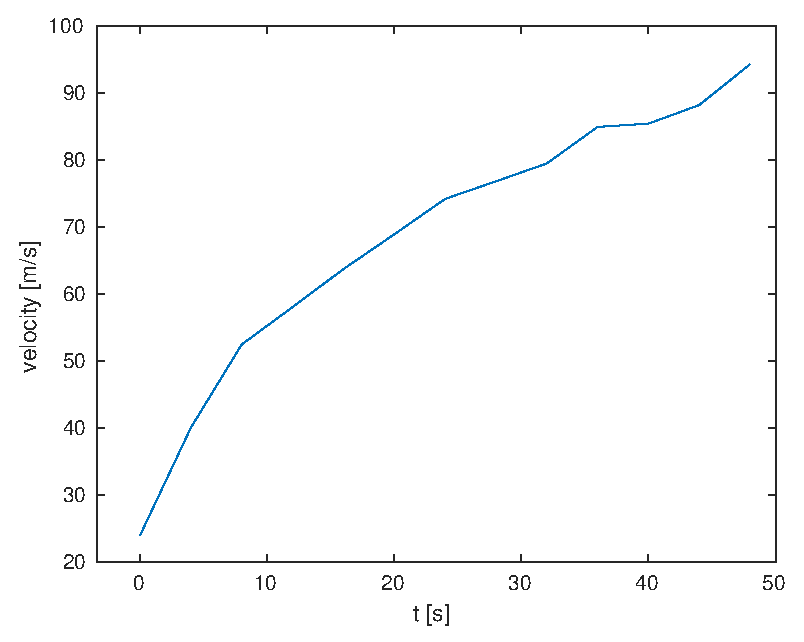
\includegraphics[width=0.8\textwidth]{img/9_1.eps}
  \captionsetup{justification=centering}
  \caption{Time versus velocity}
\end{figure}

\begin{figure}[H]
  \centering
  \includegraphics[width=0.8\textwidth]{img/9_2.eps}
  \captionsetup{justification=centering}
  \caption{Time versus acceleration}
\end{figure}



\newpage
\subsubsection{Code}
\lstinputlisting[style=Matlab-editor, basicstyle=\mlttfamily\scriptsize]{Q9.m}
\newpage
\section{Discussion}
In the discussion segment of this report, we critically analyze and reflect upon the outcomes and observations derived from the implemented numerical techniques. The Gauss quadrature’s adeptness in efficiently computing the integral is noteworthy, though a comparative analysis with the trapezoidal and Simpson's rules demonstrated that these methods, when sufficiently refined, can achieve comparable accuracy. The application of Romberg integration in rocket dynamics proved instrumental in yielding insights into its ascent, while also exhibiting the significance of adaptive quadrature methods in solving real-world problems. The heat flux analysis presented an enlightening case for the pertinence of numerical differentiation techniques, laying bare the interplay between the fin’s temperature gradient and the resultant heat flux. Notably, the implementation of these techniques requires a meticulous selection of data points to ensure precision. The examination of the aircraft's motion through finite difference approximations was enlightening; however, it is vital to acknowledge that while central difference approximations offer higher accuracy, the necessity to employ forward or backward approximations at the data endpoints can induce discrepancies. The entire analysis underscored MATLAB’s invaluable capabilities as a versatile tool for numerical analysis, and the importance of carefully selecting and tailoring methods to suit the specific nuances and demands of diverse problem sets.

\section{Conclusion}
In conclusion, this report encapsulates the versatile and indispensable nature of numerical methods in grappling with a broad spectrum of scientific problems. From integrating functions with Gauss quadrature to delving into rocket kinematics via Romberg integration, the endeavor has been not only mathematically enriching but also emblematic of the interplay between theoretical concepts and real-world applications. The thermal analysis illuminated the importance of numerical differentiation in engineering applications, whereas the aircraft motion study underscored the critical role of approximations in understanding complex physical phenomena. Throughout this exploration, MATLAB emerged as an invaluable ally, rendering computational and graphical prowess to the analysis. As we reflect upon the journey undertaken, it is imperative to recognize that, while numerical methods offer powerful tools for approximating solutions, careful consideration and judicious selection of appropriate techniques are paramount to ensuring accuracy and relevance in the ever-evolving tapestry of scientific inquiry.


\end{document}
